\documentclass[a4paper]{scrartcl}

\usepackage[utf8]{inputenc}
\usepackage[ngerman]{babel}

\usepackage{url,amssymb,mathrsfs,enumerate,dsfont}
\usepackage[space,extendedchars]{grffile}
\usepackage{verbatim}
\usepackage{listings}
\usepackage{geometry}
\usepackage{tikz}
\usepackage{etoolbox}
\usetikzlibrary{automata,arrows}
\usepackage{subfigure}
\usepackage[ngerman]{babel}
\usepackage{hyperref}
\usepackage{blindtext}
\usepackage{framed}
\usepackage{paralist}
\usepackage{multirow} 
\usepackage{amsmath}
\usepackage{algorithm}
\usepackage[noend]{algpseudocode}

\def\ojoin{\setbox0=\hbox{$\bowtie$}%
  \rule[-.02ex]{.25em}{.4pt}\llap{\rule[\ht0]{.25em}{.4pt}}}
\def\leftouterjoin{\mathbin{\ojoin\mkern-5.8mu\bowtie}}
\def\rightouterjoin{\mathbin{\bowtie\mkern-5.8mu\ojoin}}
\def\fullouterjoin{\mathbin{\ojoin\mkern-5.8mu\bowtie\mkern-5.8mu\ojoin}}

\usetikzlibrary{arrows,shapes, automata}
\setkomafont{disposition}{\normalfont\bfseries}
\setlength\parindent{0pt}

\lstset
{ %Formatting for code in appendix
    language=c,
    basicstyle=\footnotesize,
    numbers=left,
    stepnumber=1,
    showstringspaces=false,
    tabsize=4,
    breaklines=true,
    breakatwhitespace=false,
}

\title{Mathematik für Informatiker \\ Kombinatorik, Stochastik und Statistik}
\subtitle{Übungsblatt 6}
\author{Tom Paßberg , Iain Dorsch}
\date{}
\begin{document}

\maketitle
\newpage

\section*{Aufgabe 1}
Die Gewinnwarscheinlichkeit läßt sich durch $(\frac{1}{2})^n$ beschreiben. Der erwartete Gewinn kann durch die Summe der gewichteten Gewinne beschrieben werden.
Die Summe ist aufgeteilt in den Teil in dem der Gewinn variabel ist (hat noch nicht $2^{47}$ erreicht) und den Teil in dem der Gewinn aufgrund der Obergrenze konstant ist.

\begin{align}
	&\sum_{n=1}^{46} \	frac{2^n}{2^n} + \sum_{n=47}^{\infty} \dfrac{2^{47}}{2^n}\\
	= &\sum_{n=1}^{46} 1 + \sum_{n=0}^{\infty} \dfrac{2^{47}}{2^{n+47}}\\
	= &46 + \sum_{n=0}^{\infty} \dfrac{1}{2^n}\\
	= &46 + \dfrac{1}{1-\dfrac{1}{2}}\\
	= &48
\end{align}
(3) geometrische Reihe $\sum_{k=0}^{\infty} q^n = \dfrac{1}{1-q}$\\[12pt]
Der erwartete Gewinn beträgt also 48.\\
\section*{Aufgabe 2}
\subsection*{a)}
\begin{verbatim}
D1: 6, D2: 2, Sum: 8
D1: 5, D2: 1, Sum: 6
D1: 5, D2: 3, Sum: 8
Gewonnen: true, Gewinn: 1
D1: 2, D2: 1, Sum: 3
Gewonnen: false, Gewinn: 0
D1: 4, D2: 2, Sum: 6
D1: 3, D2: 4, Sum: 7
Gewonnen: false, Gewinn: -1
D1: 2, D2: 2, Sum: 4
D1: 1, D2: 2, Sum: 3
D1: 5, D2: 1, Sum: 6
D1: 5, D2: 5, Sum: 10
D1: 1, D2: 6, Sum: 7
Gewonnen: false, Gewinn: -2
D1: 2, D2: 3, Sum: 5
D1: 1, D2: 6, Sum: 7
Gewonnen: false, Gewinn: -3
D1: 2, D2: 2, Sum: 4
D1: 6, D2: 4, Sum: 10
D1: 1, D2: 2, Sum: 3
D1: 2, D2: 5, Sum: 7
Gewonnen: false, Gewinn: -4
D1: 3, D2: 3, Sum: 6
D1: 2, D2: 6, Sum: 8
D1: 3, D2: 2, Sum: 5
D1: 3, D2: 4, Sum: 7
Gewonnen: false, Gewinn: -5
D1: 6, D2: 3, Sum: 9
D1: 3, D2: 4, Sum: 7
Gewonnen: false, Gewinn: -6
D1: 2, D2: 1, Sum: 3
Gewonnen: false, Gewinn: -7
D1: 2, D2: 5, Sum: 7
Gewonnen: true, Gewinn: -6
\end{verbatim}
Mittlerer Gewinn: $ \frac{-6}{10} = -0.6$
\newpage
\subsection*{b)}
Programm in Rust:
\begin{lstlisting}
fn main() {
	let sample_size = 1000;
	
	let money: i64 = (0..sample_size)
		.map(|_| match roll_dice(2) {
			7 | 11 => 1,
			2 | 3 | 12 => -1,
			s => loop {
				match roll_dice(2) {
					7 => return -1,
					n => if n == s { return 1; }
				}   
			}
		})
		.sum();

	println!("Mittlerer Gewinn: {:.2}",money as f64/sample_size as f64)
}

fn roll_dice(number: usize) -> u8 {
	(0..number).map(|_| rand::random::<u8>() % 6 + 1).sum()
}   
\end{lstlisting}
Output:
\begin{verbatim}
Mittlerer Gewinn: -0.02
\end{verbatim}
\newpage
\section*{Aufgabe 3}
\begin{figure}[h]
	\centering
	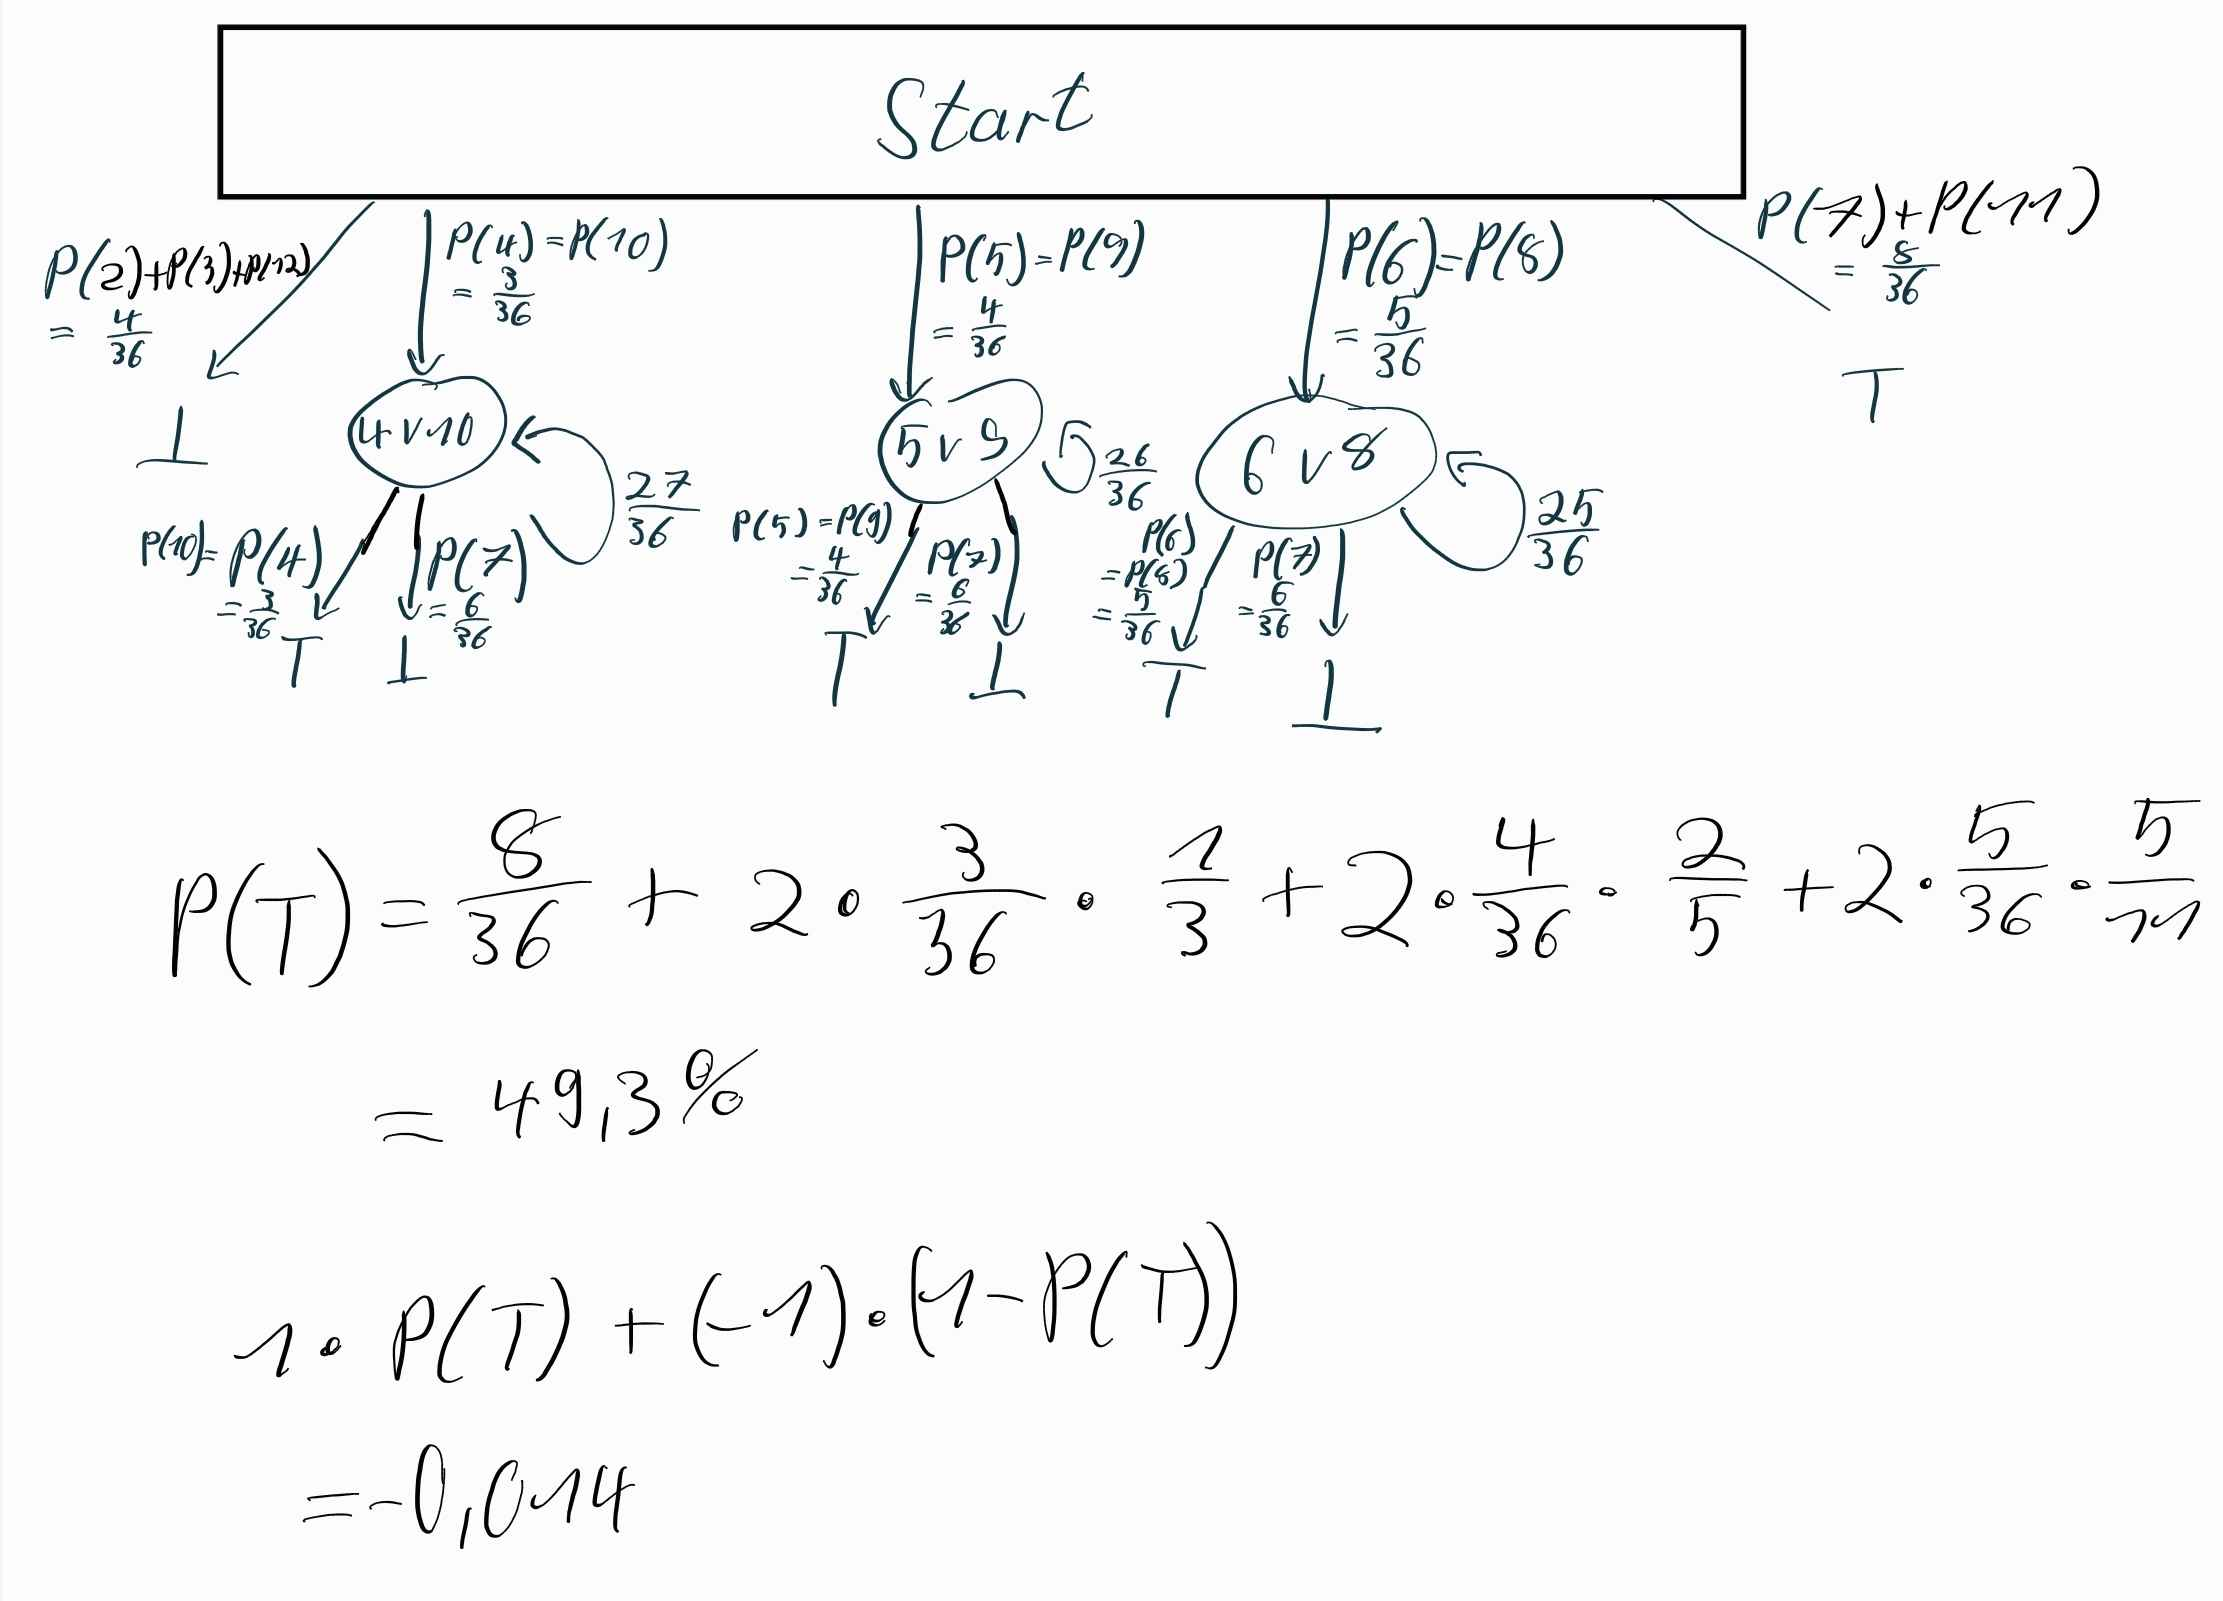
\includegraphics[width=0.95\linewidth]{./a3.jpg}
	\caption{Wahrscheinlichkeitsbaum}
	\label{fig:3}
\end{figure}


\end{document}